\section{Présentation du système}

La cellule robotique support de ce TD associe un robot SCARA, un convoyeur,
une IHM et un automate Schneider M340. Elle est décrite en détail dans le
document \emph{RIF\_GT\_TP1\_2024} fourni en support de cours ; seuls les
éléments indispensables à la compréhension du besoin sont rappelés ici.

\begin{figure}[h!]
    \centering
    \IfFileExists{imgs/vue_globale.jpg}{%
        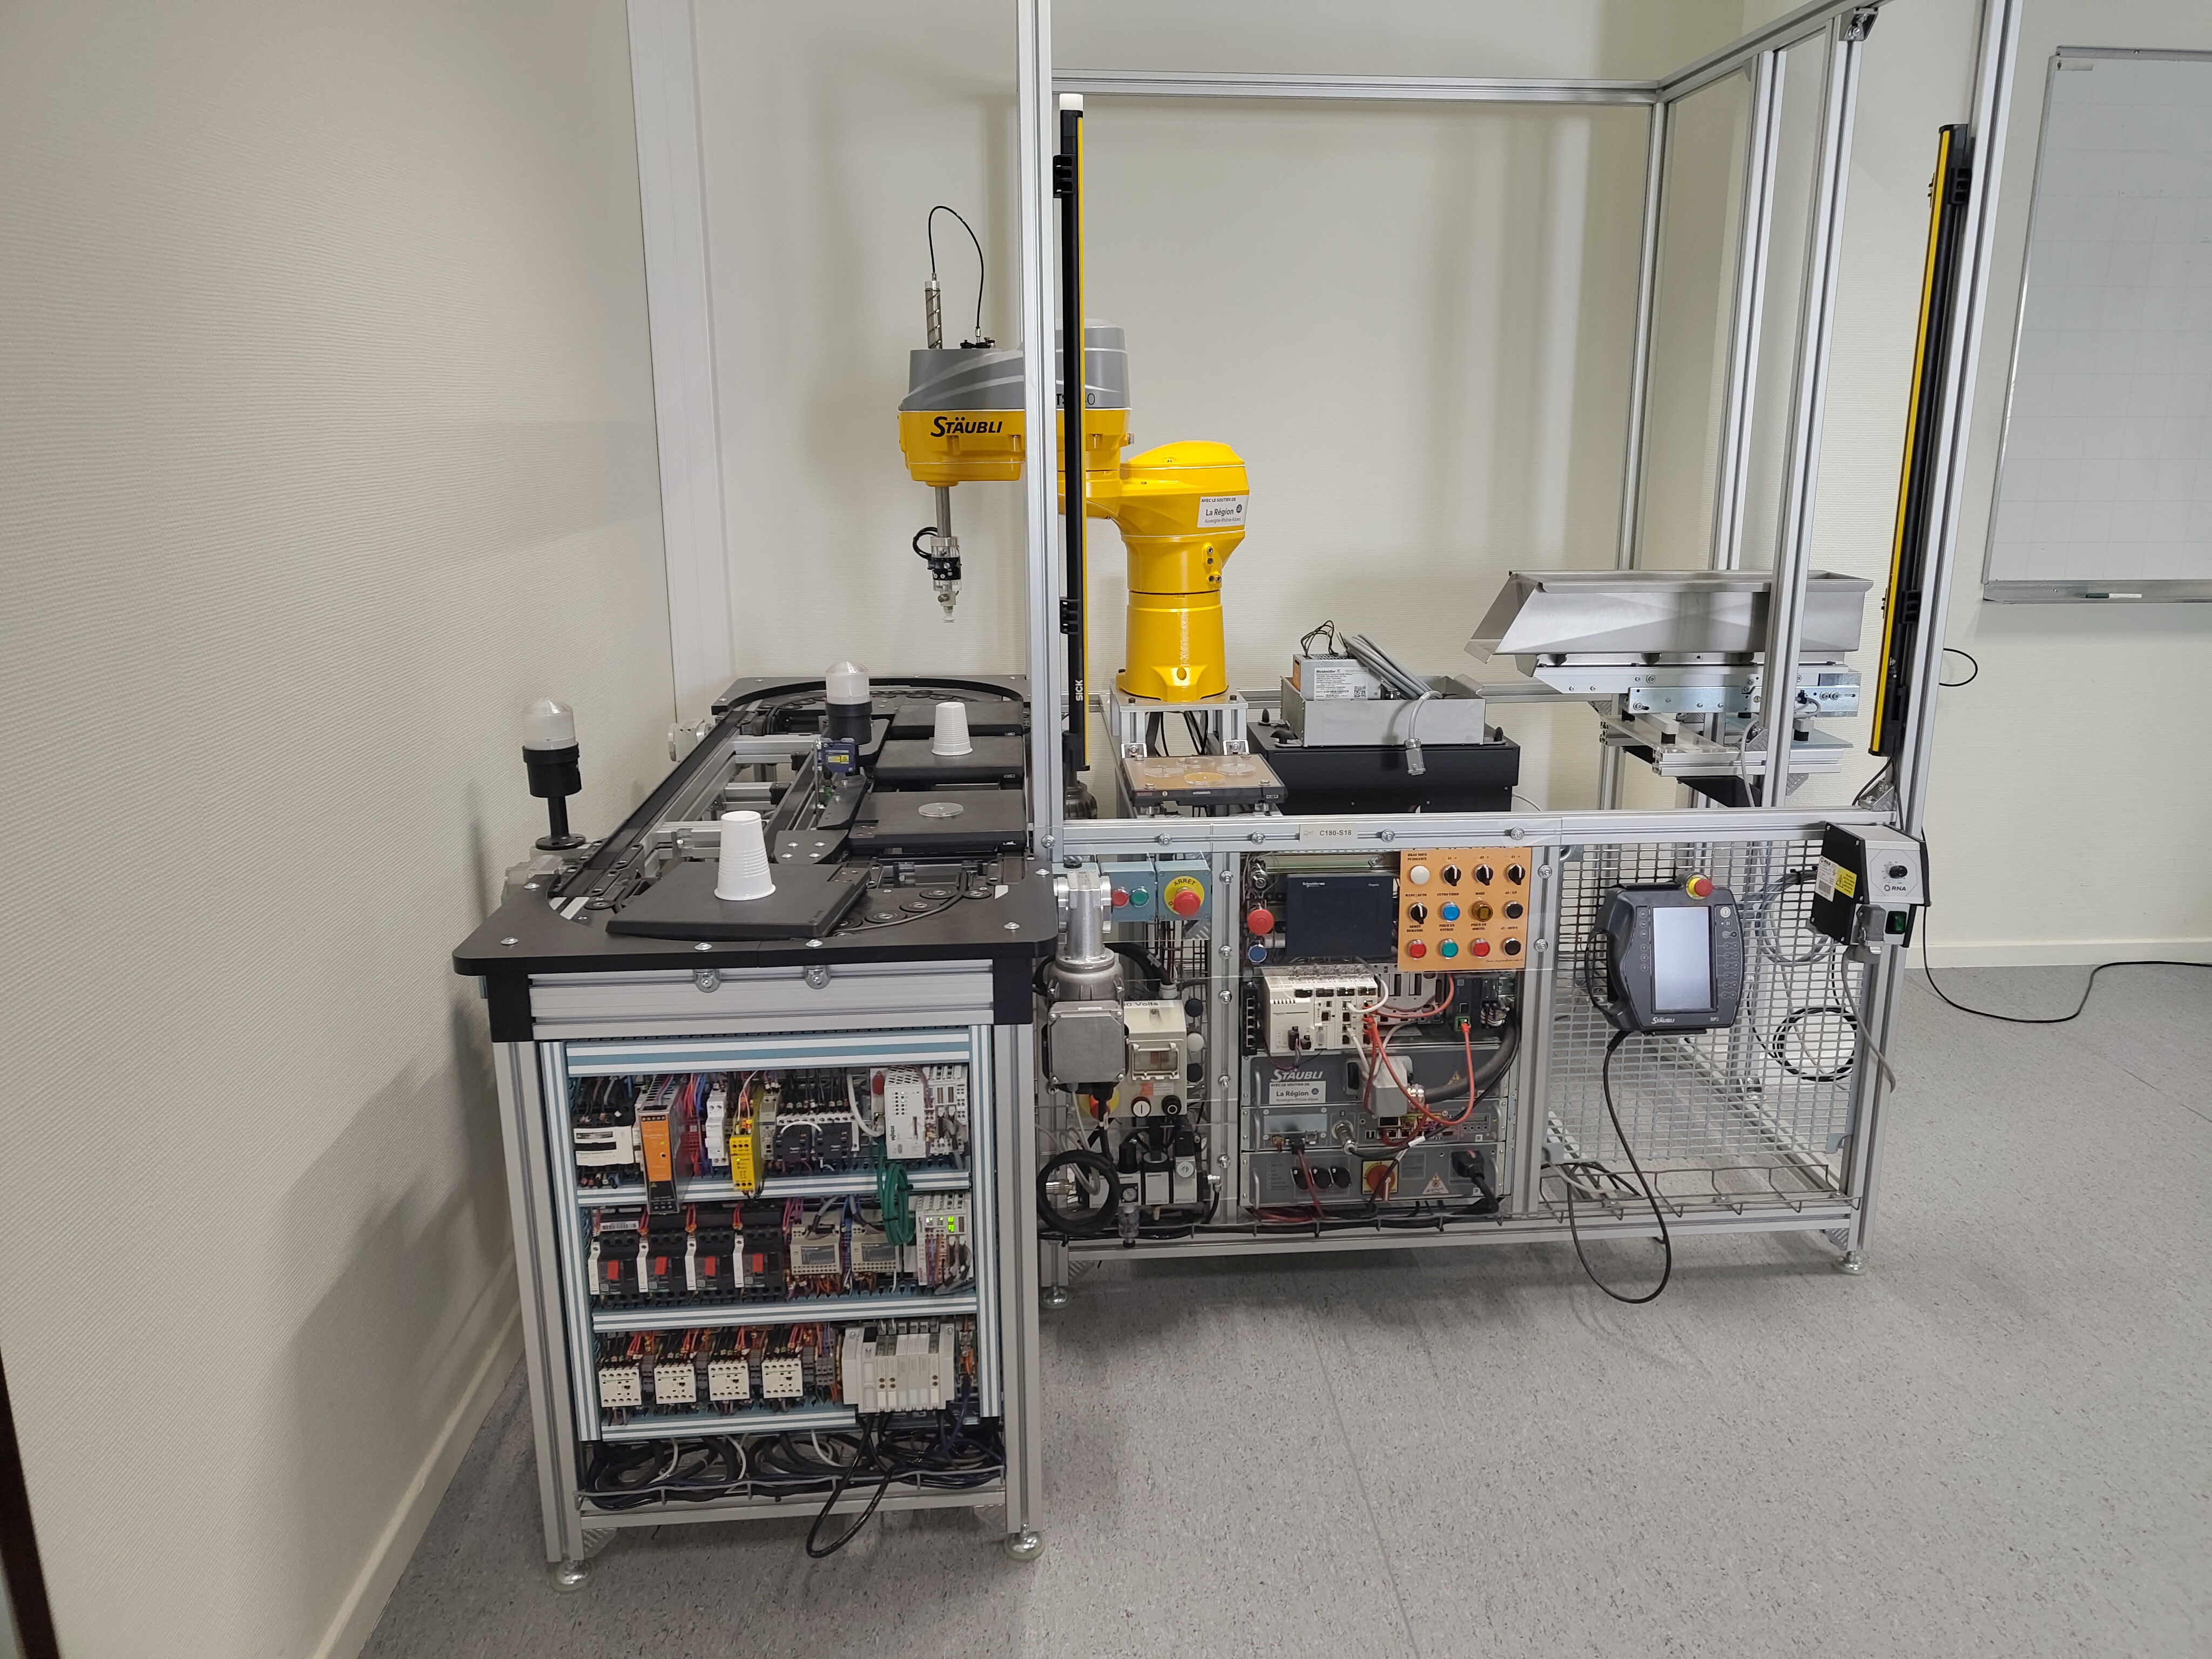
\includegraphics[width=0.8\textwidth]{imgs/vue_globale.jpg}
    }{%
        \fbox{\parbox[c][4cm][c]{0.8\textwidth}{\centering Emplacement réservé : \texttt{vue\_globale.jpg}}}
    }
    \caption{Vue globale de la cellule robotique}
\end{figure}

\begin{minipage}[t]{0.48\textwidth}
    \centering
    \IfFileExists{imgs/robot.jpg}{%
        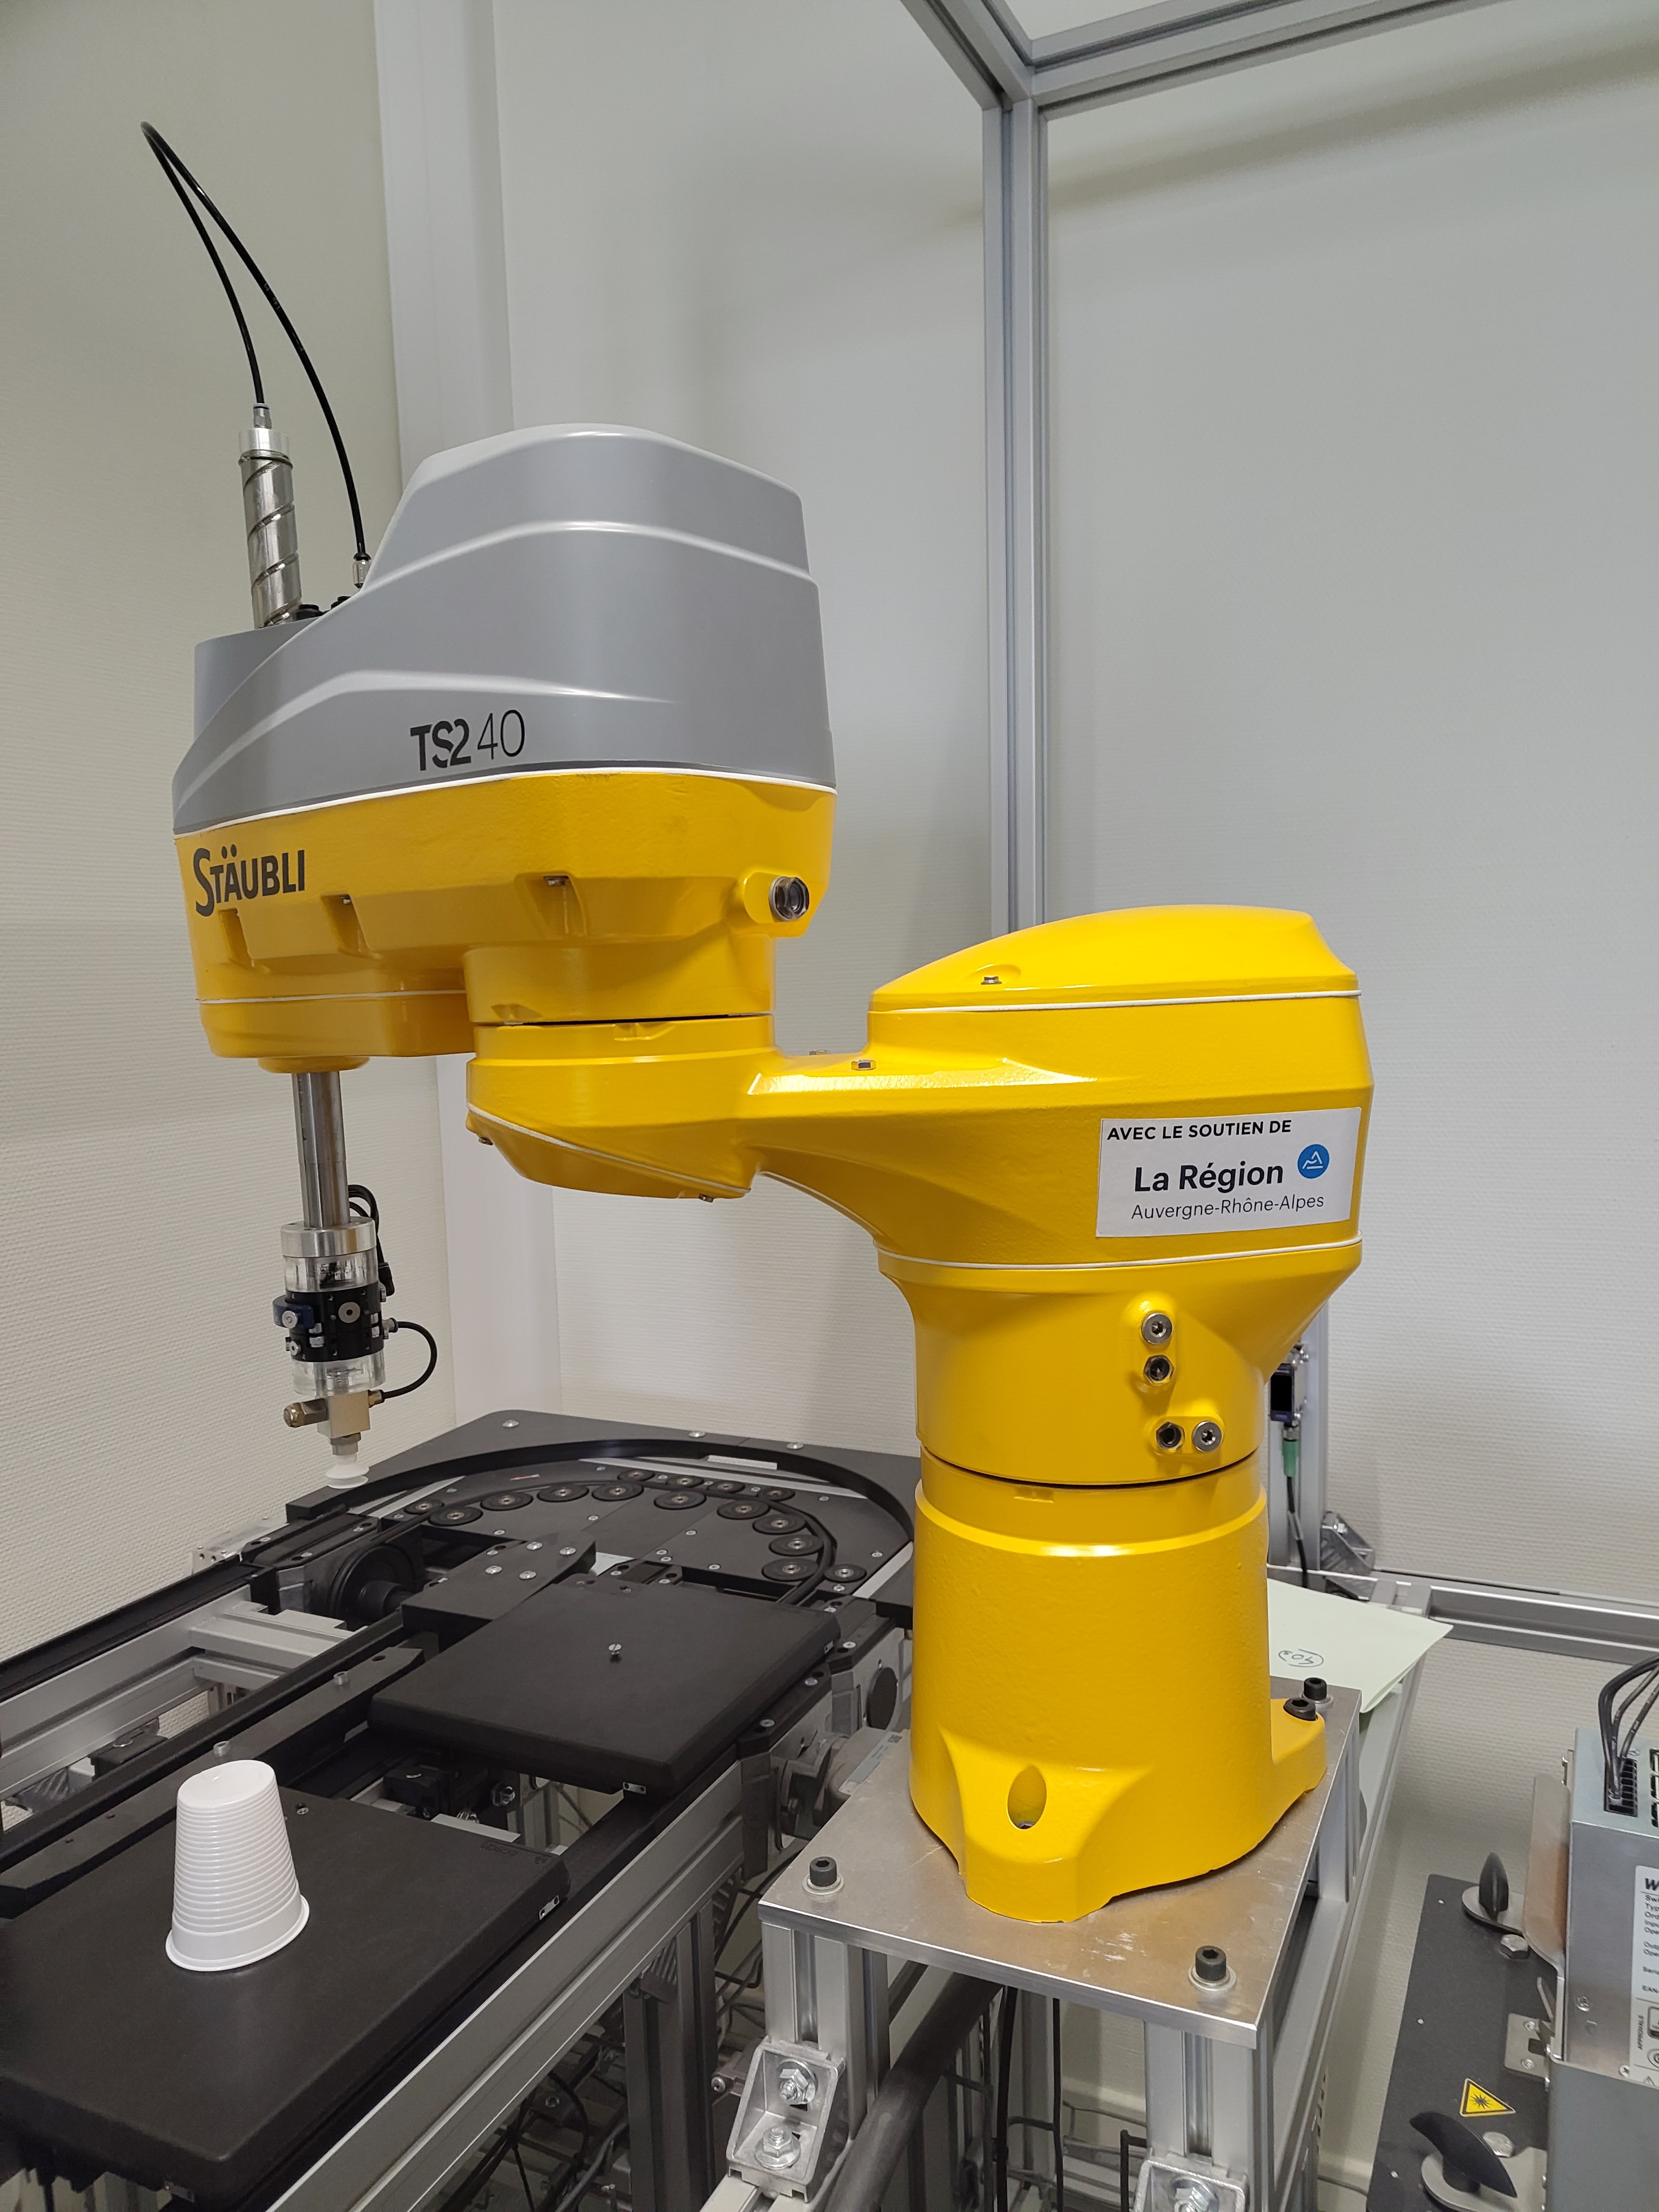
\includegraphics[width=\textwidth]{imgs/robot.jpg}
    }{%
        \fbox{\parbox[c][3cm][c]{0.9\textwidth}{\centering Emplacement réservé : \texttt{robot.jpg}}}
    }\\
    \textit{Robot SCARA}
\end{minipage}
\hfill
\begin{minipage}[t]{0.48\textwidth}
    \centering
    \IfFileExists{imgs/convoyeur.jpg}{%
        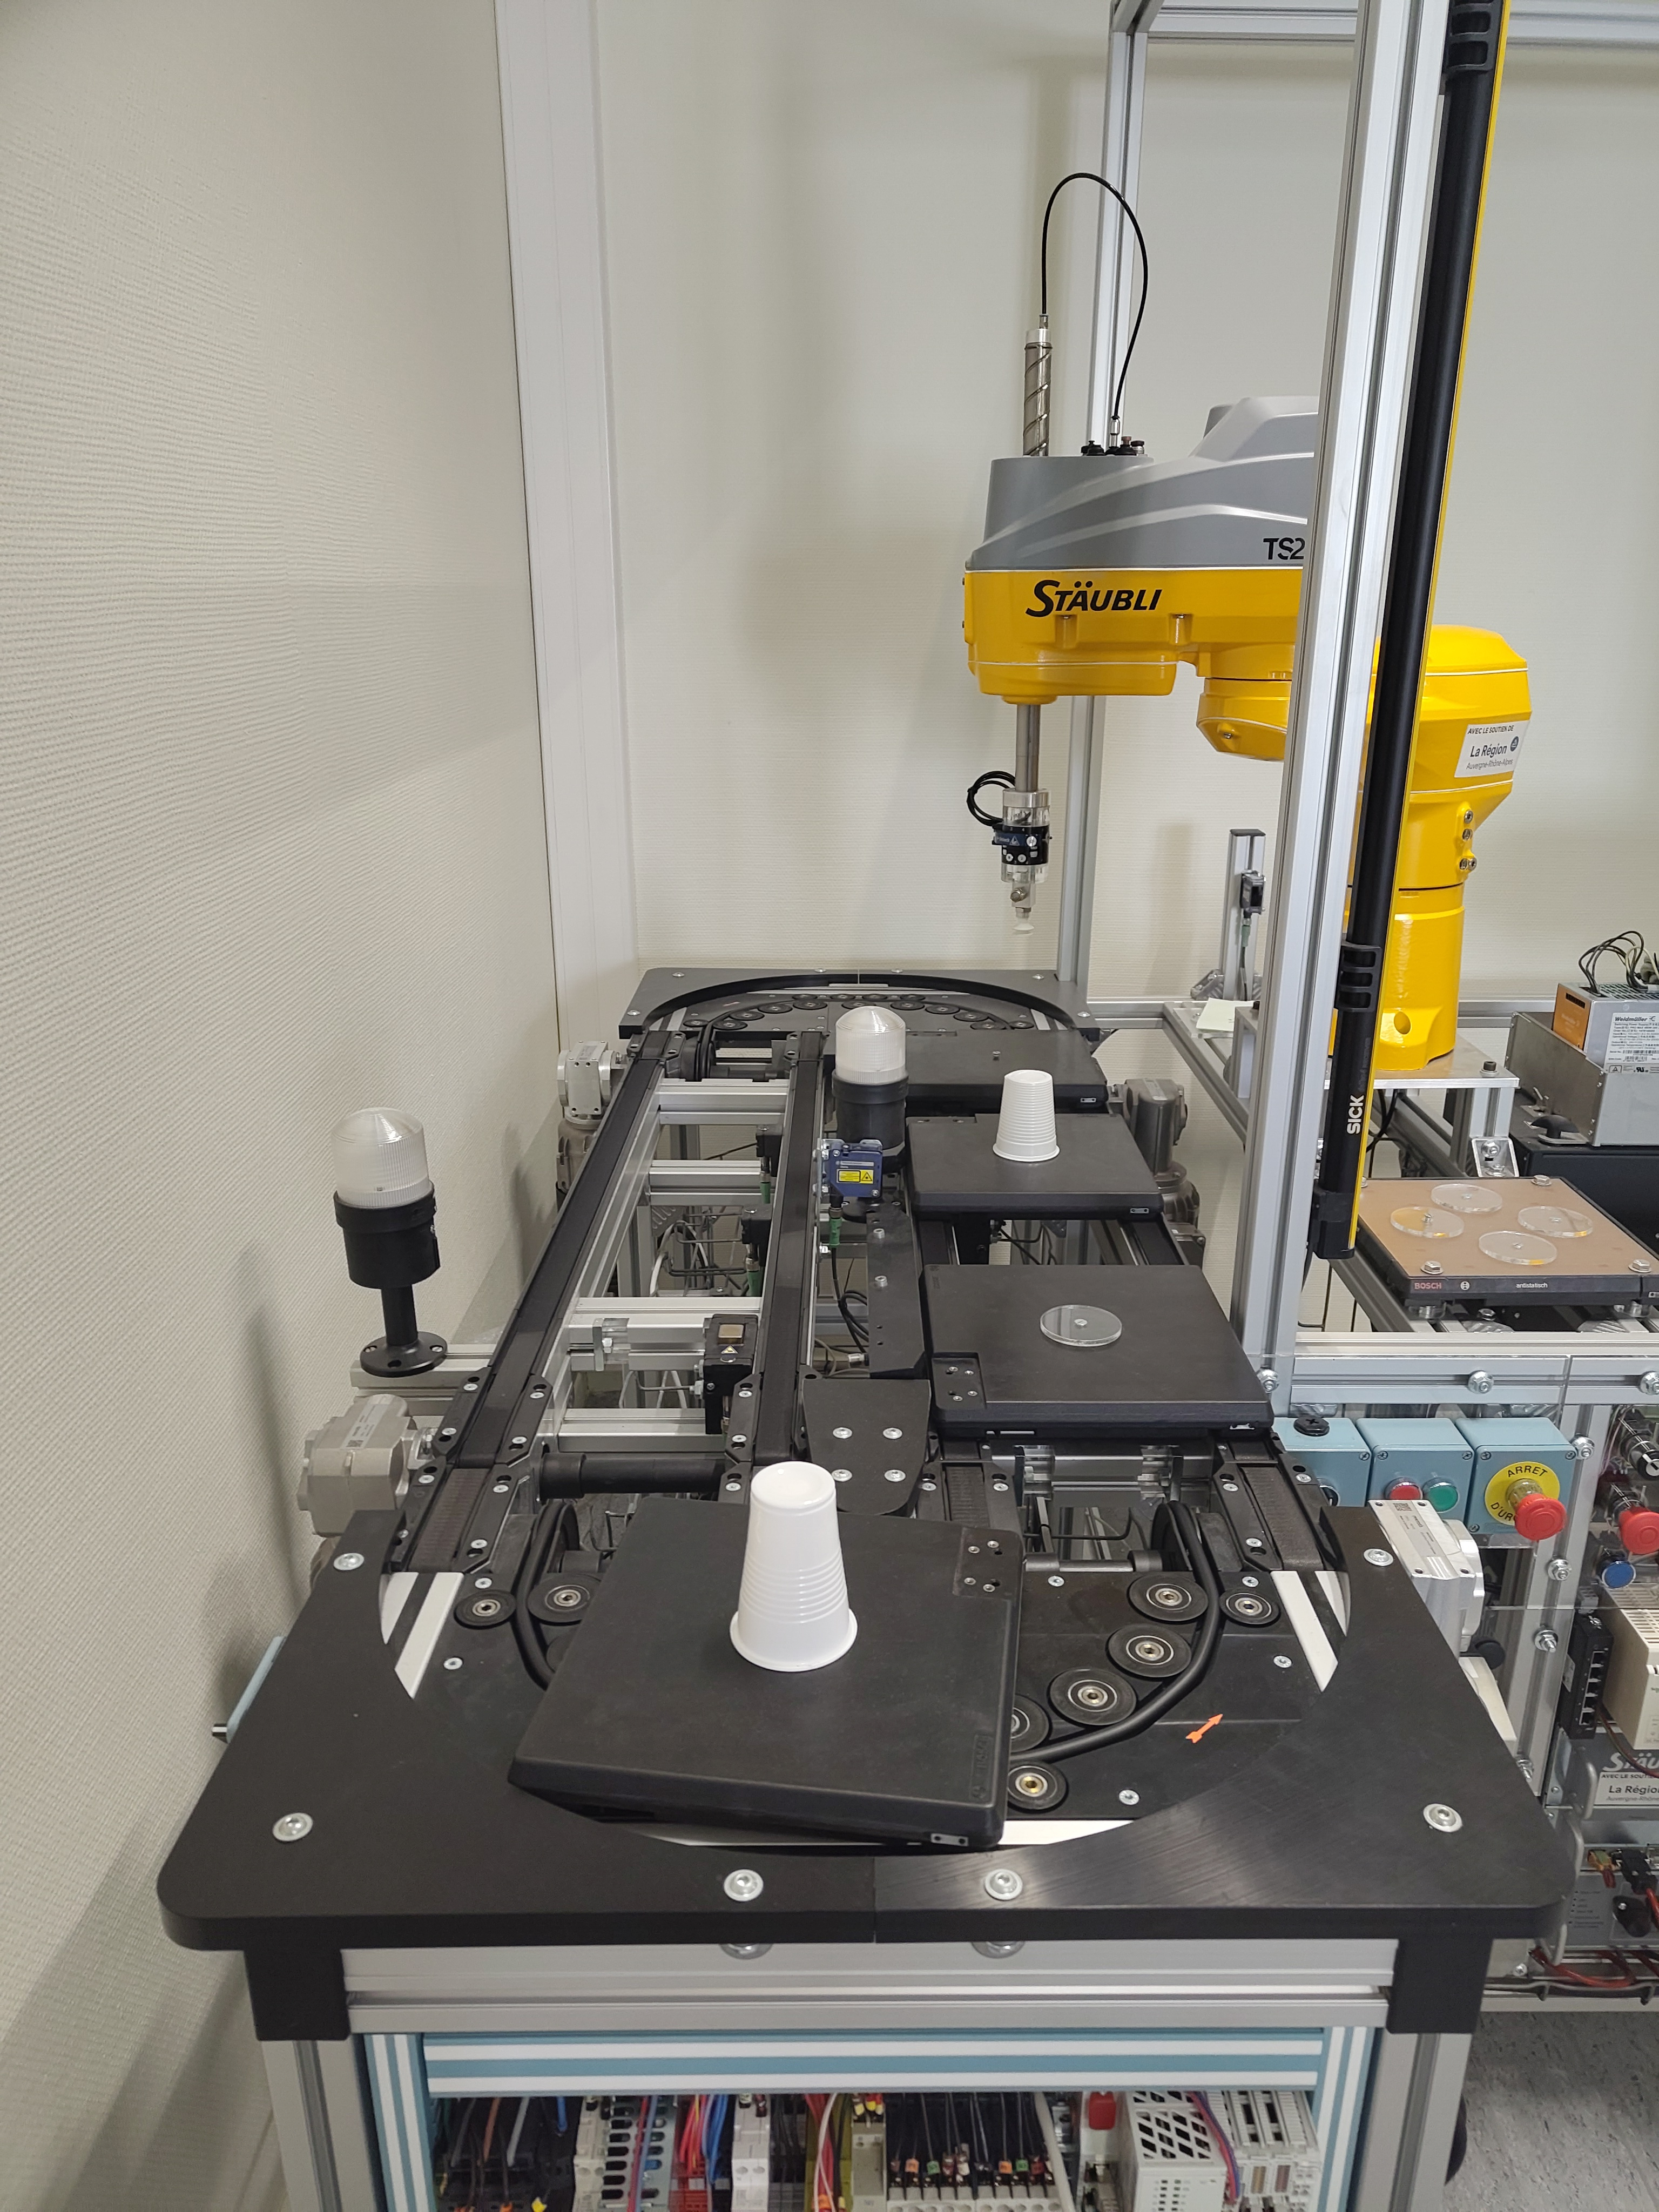
\includegraphics[width=\textwidth]{imgs/convoyeur.jpg}
    }{%
        \fbox{\parbox[c][3cm][c]{0.9\textwidth}{\centering Emplacement réservé : \texttt{convoyeur.jpg}}}
    }\\
    \textit{Convoyeur}
\end{minipage}

\vspace{0.5cm}

\begin{minipage}[t]{0.31\textwidth}
    \centering
    \IfFileExists{imgs/panneau_electrique_convoyeur.jpg}{%
        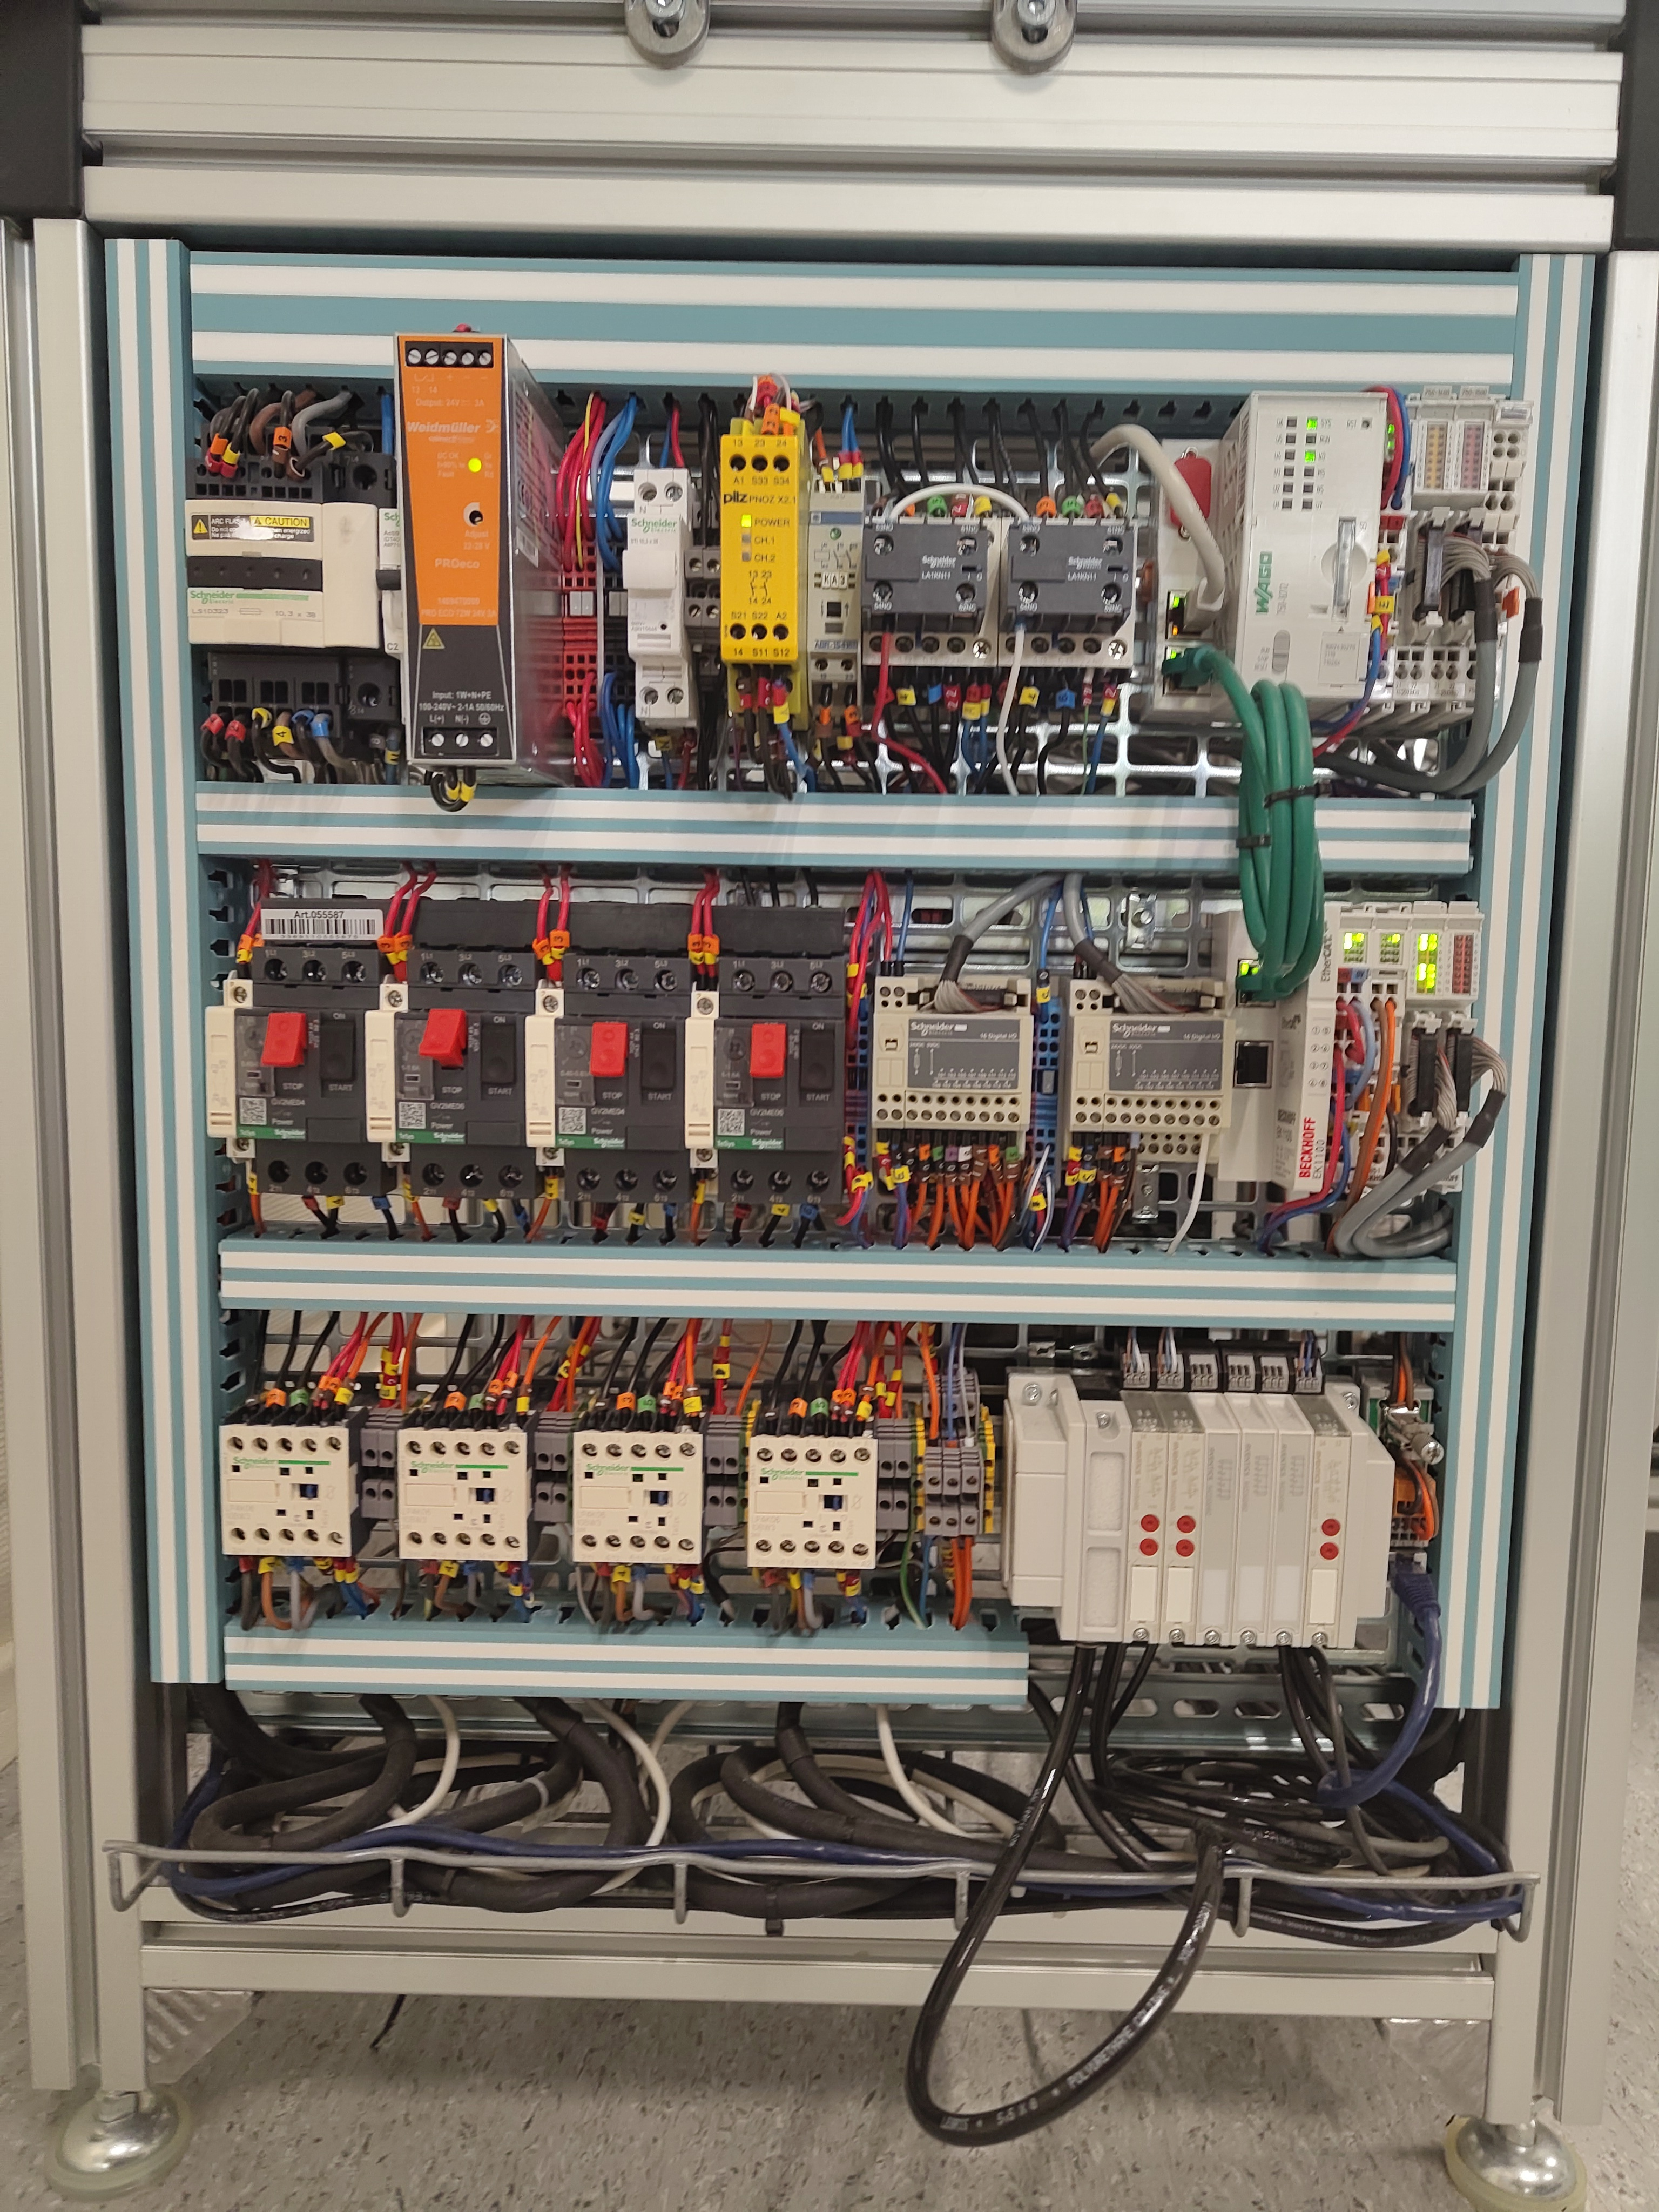
\includegraphics[width=\textwidth]{imgs/panneau_electrique_convoyeur.jpg}
    }{%
        \fbox{\parbox[c][3cm][c]{0.9\textwidth}{\centering Emplacement réservé : \texttt{panneau\_electrique\_convoyeur.jpg}}}
    }\\
    \textit{Panneau électrique du convoyeur}
\end{minipage}
\hfill
\begin{minipage}[t]{0.31\textwidth}
    \centering
    \IfFileExists{imgs/IHM.jpg}{%
        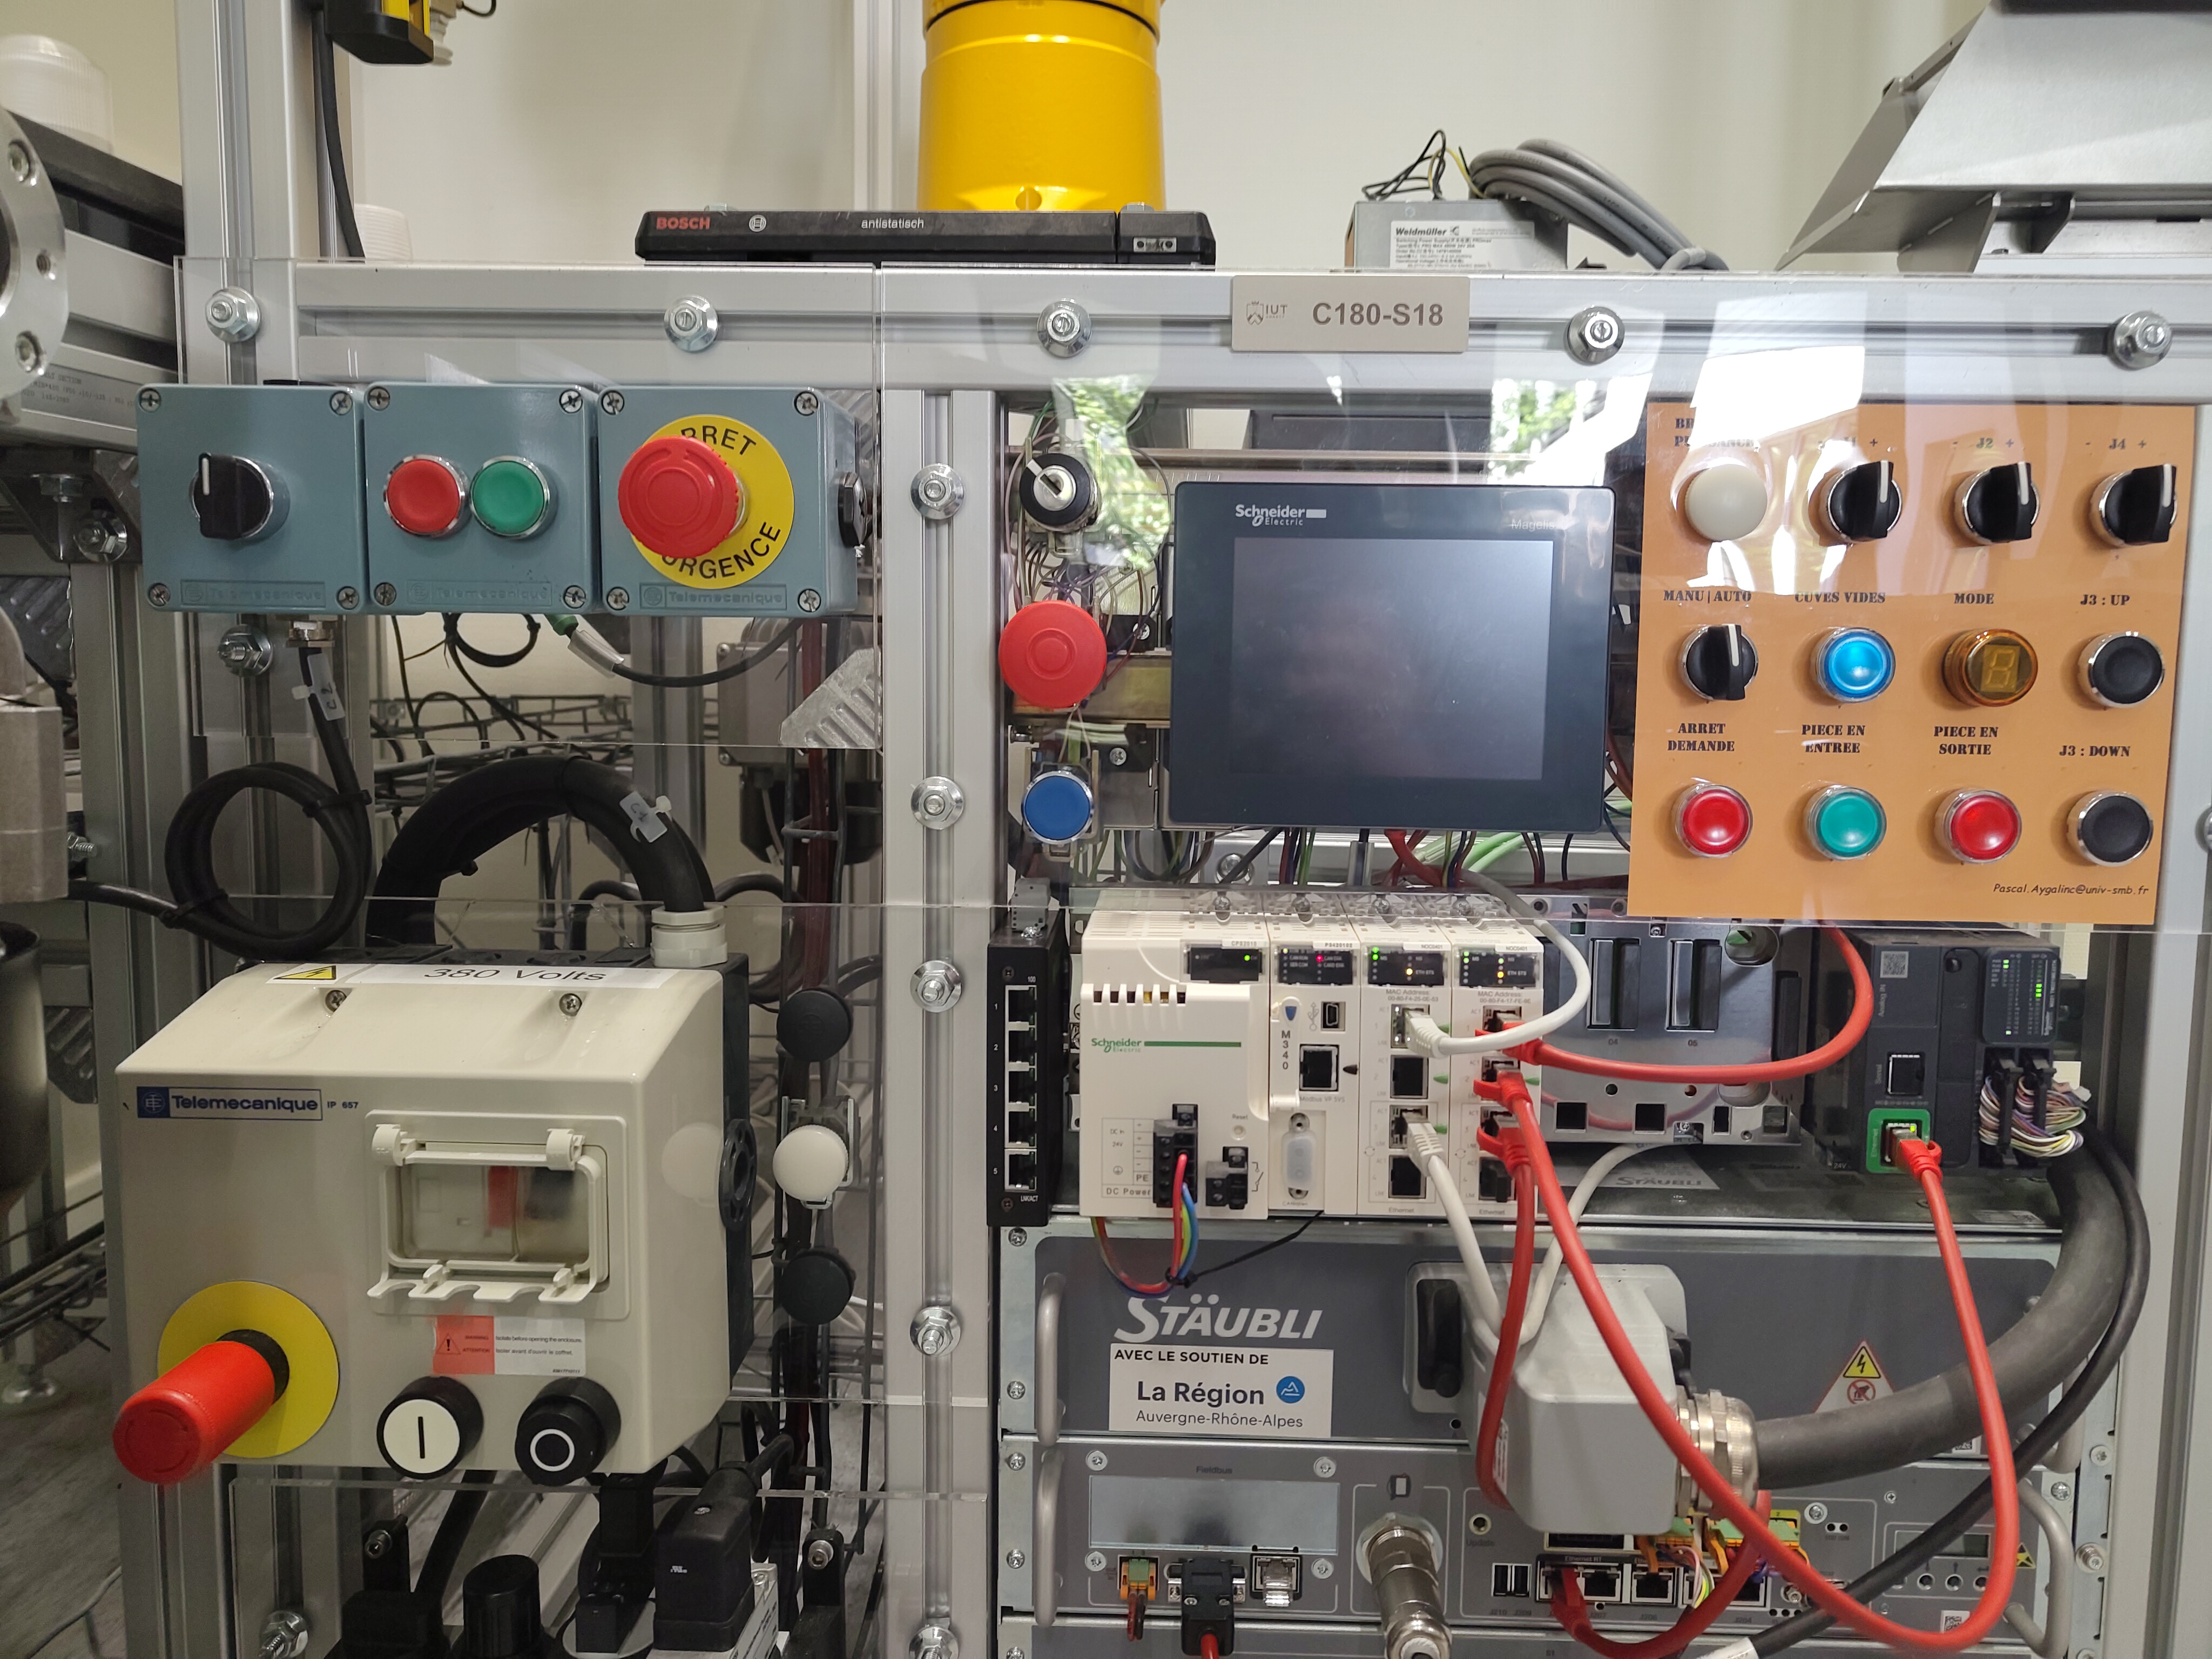
\includegraphics[width=\textwidth]{imgs/IHM.jpg}
    }{%
        \fbox{\parbox[c][3cm][c]{0.9\textwidth}{\centering Emplacement réservé : \texttt{IHM.jpg}}}
    }\\
    \textit{IHM}
\end{minipage}
\hfill
\begin{minipage}[t]{0.31\textwidth}
    \centering
    \IfFileExists{imgs/baie_cs9.jpg}{%
        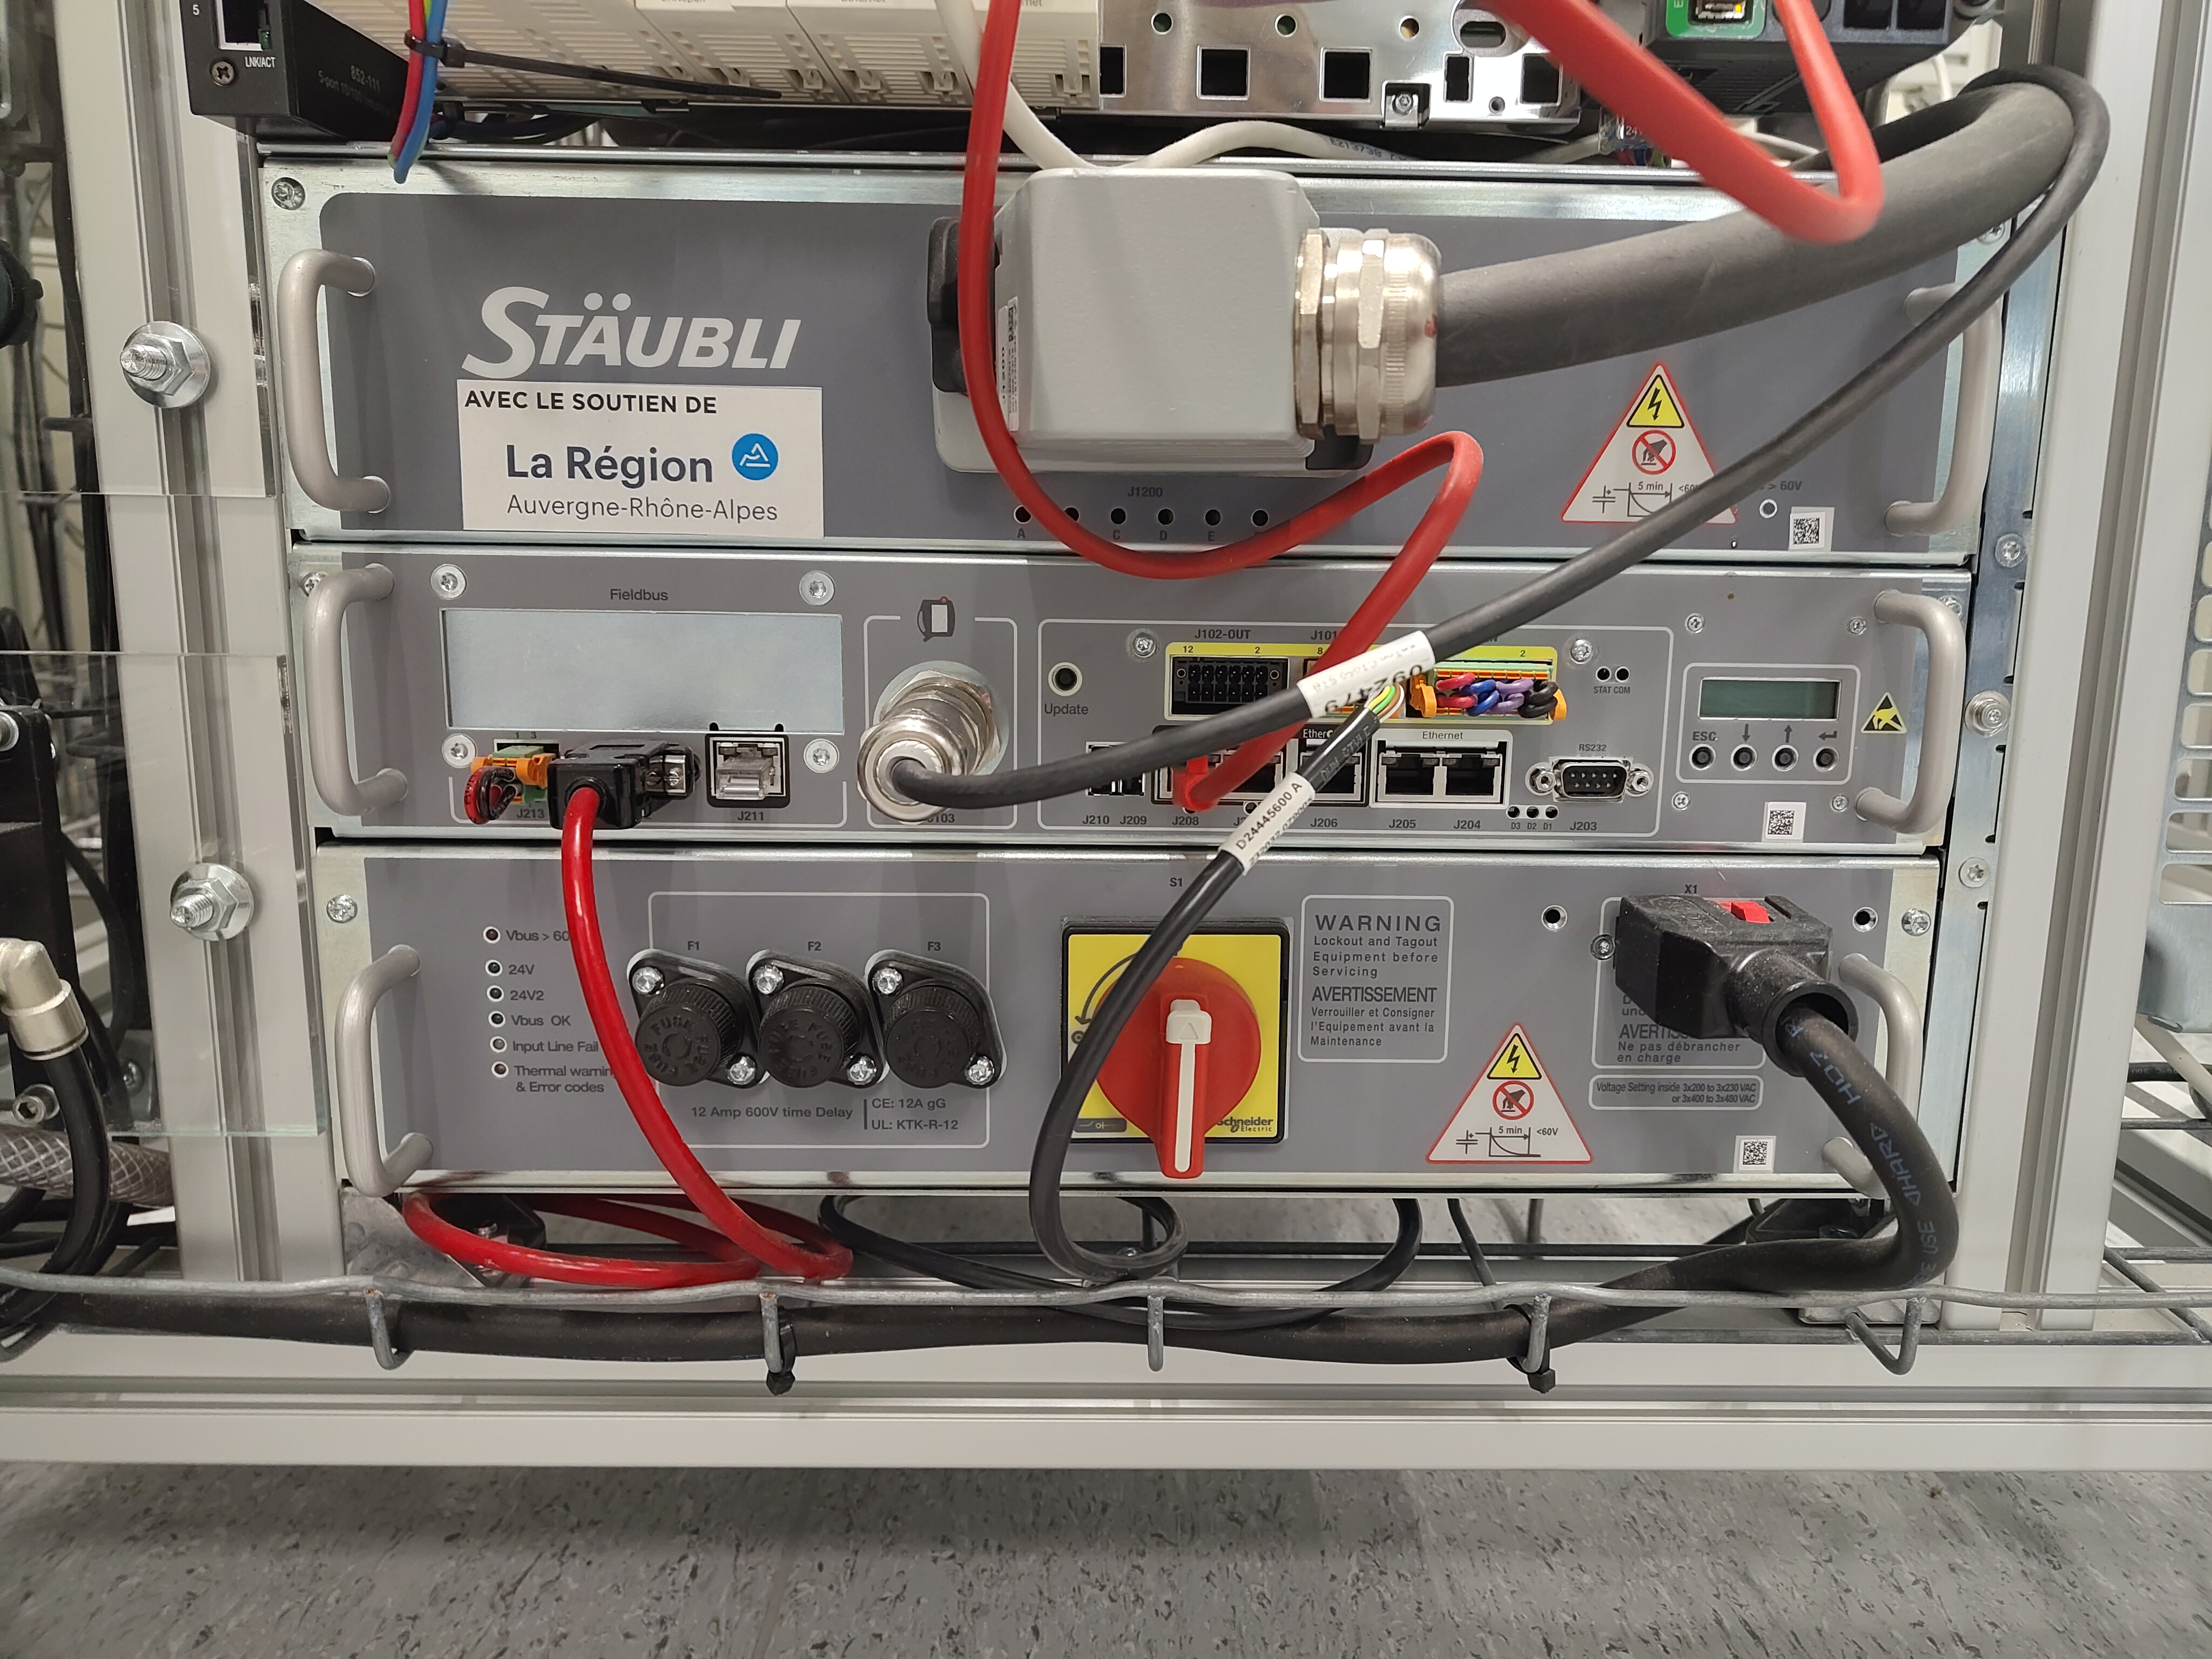
\includegraphics[width=\textwidth]{imgs/baie_cs9.jpg}
    }{%
        \fbox{\parbox[c][3cm][c]{0.9\textwidth}{\centering Emplacement réservé : \texttt{baie\_cs9.jpg}}}
    }\\
    \textit{Baie automate CS9 (M340)}
\end{minipage}

\subsection{Besoin}

On souhaite mettre en œuvre le traitement de pièces (des gobelets) par la
cellule robotique décrite ci-dessus. Le traitement consiste à faire
\textbf{tremper les gobelets dans une cuve} pendant une durée :
\begin{itemize}
    \item minimale de \textbf{10~s} ;
    \item maximale de \textbf{1~min}.
\end{itemize}

L'installation dispose de \textbf{4 cuves}, pouvant être utilisées en
parallèle pour traiter plusieurs gobelets simultanément.

La cellule est composée :
\begin{itemize}
    \item d'un robot SCARA, chargé de manipuler les gobelets (prise, dépose
    dans les cuves, évacuation) ;
    \item d'un convoyeur, assurant l'acheminement des gobelets ;
    \item d'une IHM, permettant à l'opérateur de piloter et de superviser
    l'installation ;
    \item d'un automate Schneider M340, qui coordonne l'ensemble.
\end{itemize}

\subsection{Le convoyeur et le poste guichet}

Le convoyeur assure la circulation des \textbf{palettes} portant les
gobelets. Il est supposé toujours en marche : ce sont des \textbf{bloqueurs}
répartis le long du convoyeur qui régulent le passage des palettes d'un
poste à l'autre.

Le poste qui vous intéresse plus particulièrement pour cette conception est
le \textbf{guichet} : c'est le poste d'échange entre le convoyeur et la
cellule robotisée, sur lequel le robot SCARA vient prélever ou déposer une
palette. Ce poste est équipé :
\begin{itemize}
    \item de deux bloqueurs, l'un en entrée du poste et l'autre isolant le
    poste du reste du flux de palettes ;
    \item de capteurs permettant de détecter l'arrivée d'une palette et son
    maintien en poste ;
    \item d'une colonne lumineuse (rouge/vert/bleu) qui permet de signaler
    l'état du guichet à l'opérateur (libre, en cours d'occupation, occupé,
    en cours de libération).
\end{itemize}

\begin{UPSTIwarning}{Guichet de capacité unitaire}
Le guichet fonctionne comme un \textbf{sas} : sa \textbf{capacité est
unitaire}. Il ne doit jamais recevoir plus d'une palette à la fois. Cette
contrainte, liée à la fois à l'espace de travail du robot et à la sécurité
de l'échange, doit être respectée par la commande que vous concevrez,
quel que soit le mode de fonctionnement considéré.
\end{UPSTIwarning}

C'est à votre équipe de concevoir l'architecture matérielle et logicielle
permettant de répondre à ce besoin, dans le respect des contraintes énoncées
en \cref{secContraintes}.
